\subsection{Terrein}
Het terrein kan in wezen allerlei vormen hebben, voorwaarde hierbij is dat het een eerlijk terrein is voor beide teams. Een team mag dus geen voordeel hebben dankzij de kaart. Een mogelijke manier om dit te bereiken is door de kaart symmetrisch te maken. We eisen bovendien dat de kaart rechthoekig is.

Op het terrein zijn twee commandocentra geplaatst, voor beide teams een commandocentrum. Het kan gewenst zijn dat elk team bij de start van het spel ook al een aantal extra torens heeft ter bescherming van het commandocentrum. Over het terrein zijn een aantal delfplaatsen verdeeld. Deze zijn eerlijk verdeeld over de kaart. Andere obstakels mogen aanwezig zijn, maar zijn niet noodzakelijkerwijs aanwezig. Alle objecten met uitzondering van spelers worden geplaatst op een rooster. In figuur \ref{fig:map1} en \ref{fig:map2} zijn twee mogelijke beginconfiguraties van het spel getoond.
\begin{figure}[h]
\begin{subfigure}{0.5\textwidth}
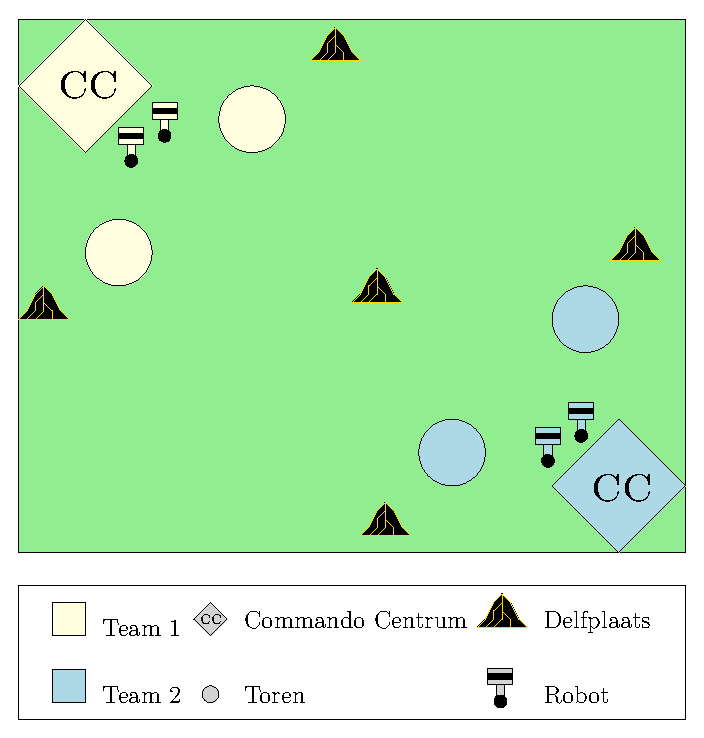
\includegraphics[width=\textwidth]{Graphics/Map1.eps}
\caption{Een bijna vierkant terrein met vier spelers}
\label{fig:map1}
\end{subfigure}\hspace{10mm}
\begin{subfigure}{0.5\textwidth}
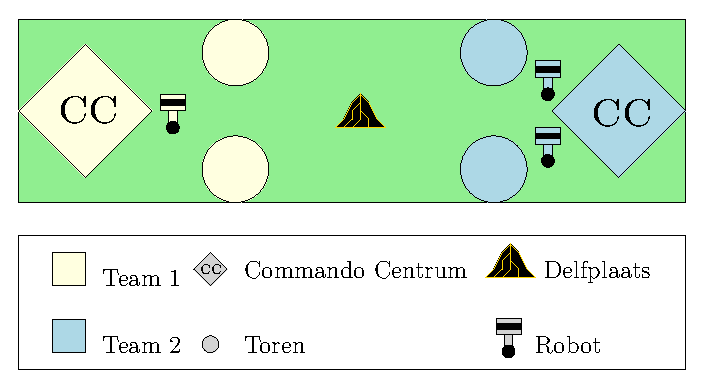
\includegraphics[width=\textwidth]{Graphics/Map2.eps}
\caption{Een breed terrein met drie spelers}
\label{fig:map2}
\end{subfigure}
\caption{Twee verschillende beginconfiguraties van het spel}
\end{figure}

\subsection{Spelers}
Een speler behoort tot \'e\'en van beide teams, spelers van een bepaald team zijn te identificeren door kleuren. De speler ziet de wereld vanuit de positie van zijn robot. Men kan de kijkrichting aanpassen, zodat deze elke willekeurige richting kan zijn. Als de kijkrichting verder naar links of rechts wordt gedraaid, draait de robot mee. Wanneer de kijkrichting hoger of lager wordt, draait de robot niet mee, het geweer zou eventueel wel mee kunnen draaien in de kijkrichting. De speler heeft een lasergeweer waarmee hij op andere spelers en torens kan schieten om deze te vernietigen. Het lasergeweer schiet laserstralen, die een oneindige snelheid hebben. Als een speler schiet, dan wordt geschoten in de huidige kijkrichting van de robot. Dit wordt verder gespecificeerd in de sectie \ref{sec:UI}: \emph{Gebruikersomgeving}. Bij het begin van het spel heeft de robot nog een volledig harnas. Zodra de speler wordt geraakt, wordt de conditie van het harnas slechter. Het is echter niet mogelijk dat een speler het harnas van een andere speler uit hetzelfde team beschadigt.
\FloatBarrier
Een speler gaat dood als zijn harnas kapot is. In dat geval zal hij na een bepaalde hoeveelheid tijd terugkeren bij het commandocentrum met een volledig harnas. De conditie van het harnas kan op geen enkele andere dan de hierboven beschreven manieren veranderen. Ook kan een speler gebouwen bouwen, hiervoor gebruikt hij goud uit de kas van het team. De spelers kunnen op het grondvlak bewegen met een vaste snelheid in elke richting. De enige voorwaarde hierbij is dat de spelers op de kaart blijven en niet door een gebouw lopen. Het is dus wel mogelijk dat spelers door elkaar heen kunnen lopen. De speler kijkt vanuit een derde persoon perspectief. In een derde persoon perspectief wordt de sc\`ene bekeken vanaf een punt vlak achter de speler.
Het is eventueel mogelijk om dit verder uit te breiden, zodat de speler kan wisselen van derde persoon perspectief naar eerste persoon perspectief.

\subsection{Gebouwen}
Er zijn drie soorten gebouwen: torens, mijnen en commandocentra. Torens schieten op spelers en andere gebouwen in hun bereik. Mijnen kunnen over delfplaatsen worden gebouwd met het doel de inkomsten van een team te vergroten. In principe levert elke mijn een vaste hoeveelheid goud voor de gezamenlijke kas op. Deze hoeveelheid wordt periodiek toegevoegd aan de kas.

Uit sommige delfplaatsen kan maar een bepaalde hoeveelheid goud worden gehaald, daarna is de delfplaats op. Dan zal de mijn over die delfplaats geen verdere bijdrage meer leveren voor de gezamenlijke kas. We staan echter ook delfplaatsen toe die een onbeperkte hoeveelheid goud bevatten. Standaard levert elke mijn hetzelfde bedrag op met dezelfde periode, maar dit kan later nog worden aangepast.

Een commandocentrum is het belangrijkste gebouw voor het team. Als dit gebouw kapot is, heeft het bijbehorende team verloren. Gebouwen kunnen door spelers worden beschoten, waardoor deze worden beschadigd. Gebouwen kunnen op geen enkele mogelijke manier hersteld worden. Optioneel zou men mechanismen in het spel kunnen toevoegen om deze gebouwen te herstellen. Alle gebouwen behoren tot \'e\'en van beide teams, deze gebouwen kunnen weer ge\"identificeerd worden door de kleur van het gebouw.

\subsection{Verzamelbare voorwerpen}
Er is maar \'e\'en verzamelbaar voorwerp: een muntje. E\'en of meerdere muntjes worden achtergelaten door spelers die dood gaan en torens die worden vernietigd. Een muntje heeft een bepaalde waarde in goud. De waarde van de muntjes zijn proportioneel aan de gezamenlijke kas van het team waarvan de speler is doodgegaan. Als een toren is vernietigd, dan is de waarde van de muntjes proportioneel aan de kosten van de toren. De waarde van de muntjes moet echter altijd kleiner zijn dan de kosten van de toren. Gedurende een spel moeten deze proporties vast zijn.

Als een speler doodgaat, wordt bovendien nog de waarde van de muntjes afgetrokken van de gezamenlijke kas van die speler. Een muntje kan vervolgens opgepakt worden door alle spelers. Het muntje is dus het voedsel element in ons spel. De waarde van het muntje zal dan toegevoegd worden aan de kas van het bijbehorende team.

\subsection{Initialisatie}
De spelers kunnen zelf kiezen bij welk team ze gaan, onder de voorwaarde dat elk team minstens \'e\'en speler heeft. Bij de start van het spel staan alle spelers bij het commandocentrum. Zoals al eerder gezegd, hebben alle spelers dan nog een volledig harnas. Bovendien heeft elk team een zekere positieve hoeveelheid goud in de gezamenlijke kas, die voor beide teams natuurlijk gelijk moet zijn. Er kunnen minstens twee mijnen gebouwd worden met deze hoeveelheid goud.
\FloatBarrier

\section{Gebruikersomgeving}
\label{sec:UI}

Via de gebruikersomgeving kan de speler de interactie met het 3D-model aangaan. De volgende componenten worden weergegeven in de User Interface tijdens het spel:
\begin{itemize}
\item De hoeveelheid goud van het team.
\item De sterkte van het harnas.
\item Het vizier van de speler.
\end{itemize}

De hoeveelheid goud van het team wordt weergegeven met behulp van een getal na een speciaal symbool linksboven: een goudstaaf. De sterkte van het harnas geven wij ook linksboven weer: de sterkte van het harnas wordt gerepresenteerd met een statusbalk. Hoe voller de balk is, hoe sterker het harnas is. We eisen dat dit verband recht evenredig is. Hierbij representeert een volle balk dat de speler nog een volledig harnas heeft. Als de balk leeg is, gaat de speler dood.

We plaatsen het vizier van de speler altijd in het midden van het scherm. Hierdoor weet de speler dus in welke richting wordt geschoten. De speler wordt altijd iets links van dit vizier getekend. Voor de duidelijkheid hebben wij hier ook een figuur van gemaakt. Een plattegrond van de kaart, zoals wordt besproken in het sectie \ref{sec:OPT}: \emph{Optioneel}, wordt ook aangegeven in figuur \ref{fig:UI}.
\begin{figure}[H]
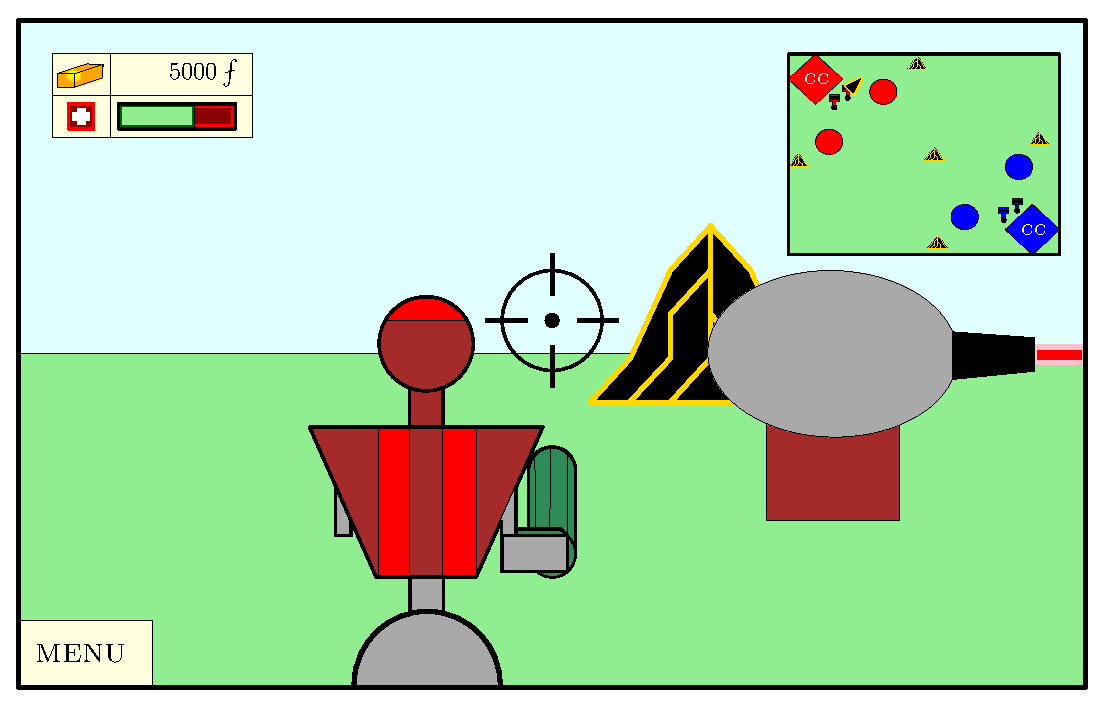
\includegraphics[width=\textwidth]{Graphics/UI.eps}
\caption{De gebruikersomgeving tijdens het spel}
\label{fig:UI}
\end{figure}
De besturing van de robot kan met de \textsc{wasd}-toetsencombinatie of door gebruik te maken van de pijltjes-toetsen. Hiervoor geven we de volgende tabel:
\begin{table}[H]
        \small
        \centering
        \begin{tabular}{| l | l |}
        \hline
        Knop & Reactie \\ \hline
        \textsc{w} of $\uparrow$ & De robot beweegt, indien mogelijk, vooruit naar de huidige kijkrichting toe \\ \hline
        \textsc{a} of $\leftarrow$ & De robot draait naar links \\ \hline
        \textsc{s} of $\downarrow$ & De robot beweegt, indien mogelijk, achteruit van de huidige kijkrichting af \\ \hline
        \textsc{d} of $\rightarrow$ & De robot draait naar rechts \\ \hline
        \end{tabular}
        \caption{Knoppen met bijbehorende reactie}
        \label{tab:planning}
    \end{table}

De speler kan schieten door op de muis te drukken. Door de muis naar boven te bewegen, kijkt de speler verder omhoog. Merk op dat het vizier altijd in het midden van het scherm blijft. De speler ziet dit dus doordat de horizon omlaag of omhoog schuift.
\FloatBarrier
\subsection{Schieten met het lasergeweer}
Men kan opmerken uit figuur \ref{fig:UI} dat de schietrichting niet meteen duidelijk uit de gebruikersomgeving wordt. Immers, het vizier wordt niet op hetzelfde punt als het wapen op het scherm afgebeeld. Aangezien, het vizier eenvoudiger is om mee te richtens dan het wapen, wordt bij het schieten een laserstraal afgevuurd vanuit het wapen naar het punt waar de vizier op gericht staat. Dit is te zien in figuur \ref{fig:COL}.
 
\begin{figure}[H]
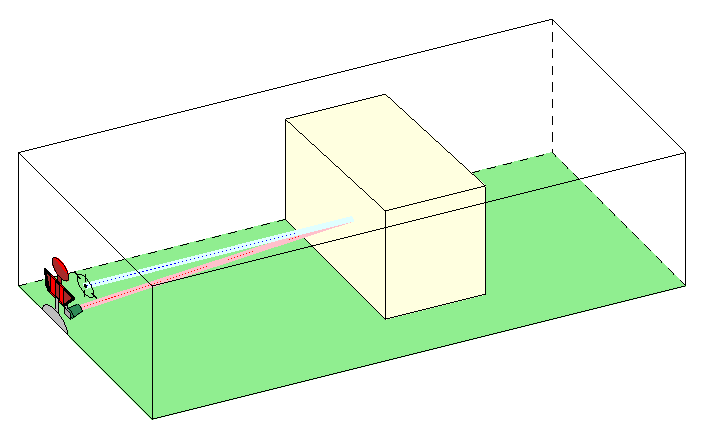
\includegraphics[width=\textwidth]{Graphics/Collision.eps}
\caption{Een voorbeeld van het schieten van het wapen}
\label{fig:COL}
\end{figure}


Een probleem hierbij, is dat een object in het pad van het wapen naar het punt, dat de vizier aanwijst, blokkeert. Er zijn twee manieren om dit op te lossen, men kan zeggen dat de laser altijd het punt van de vizier raakt. Dit is makkelijker te implementeren, aangezien we maar \'e\'en keer hoeven te bepalen waar een lijn een object raakt. Dit is te zien in figuur \ref{fig:COL2}. Een andere oplossing is dat in dit geval de laser alleen het object, dat in de weg staat, raakt. Dit is natuurlijk realistischer, maar minder makkelijk te implementeren. Dit is te zien in figuur \ref{fig:COL3}. In eerste instantie kiezen wij voor de eerste methode. Echter, indien de tijd ons de mogelijkheid gunt om de tweede oplossing te kunnen implementeren, zullen wij de tweede oplossing implementeren.
\FloatBarrier
\begin{figure}[h]
\begin{subfigure}{0.5\textwidth}
\centering
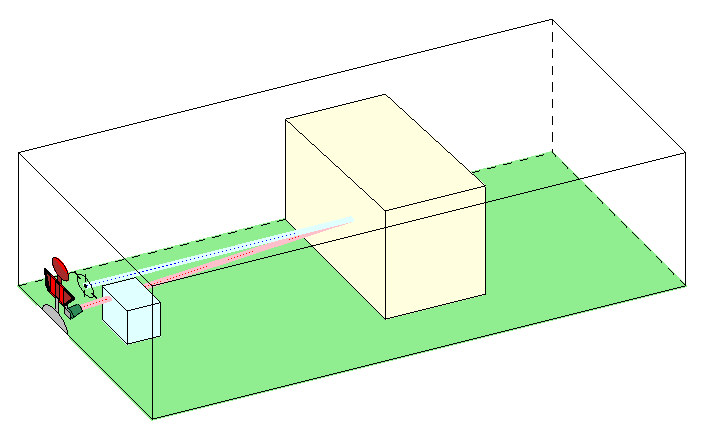
\includegraphics[width=\textwidth]{Graphics/Collision2.eps}
\caption{De laser komt altijd aan op het punt aangewezen door het vizier}
\label{fig:COL2}
\end{subfigure}
\begin{subfigure}{0.5\textwidth}
\centering
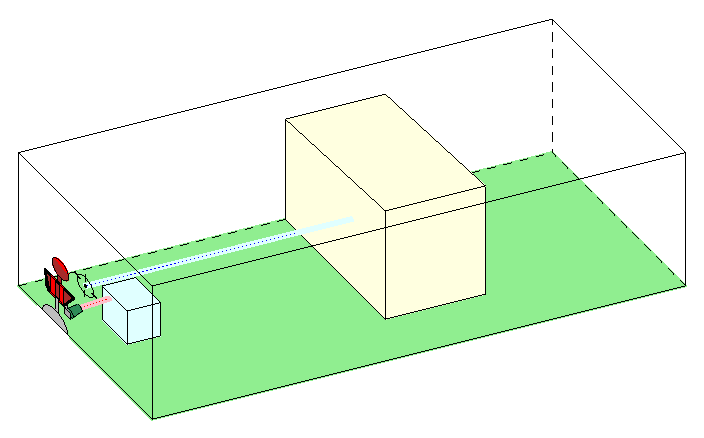
\includegraphics[width=\textwidth]{Graphics/Collision3.eps}
\caption{De laser stopt zodra hij een ander object raakt}
\label{fig:COL3}
\end{subfigure}
\end{figure}
\FloatBarrier
\section{Optioneel}
\label{sec:OPT}
We hebben ook een aantal plannen voor uitbreiding van het spel. De volgende idee\"en zouden wij graag extra implementeren. De idee\"en zijn gesorteerd op aflopende volgorde van belangrijkheid.

\begin{itemize}
  \item Extra goud, de gezamenlijke kas wordt periodiek met een vaste hoeveelheid verhoogd. Dit is dan additief met eventuele mijnen. Wij verwachten dat dit weinig tijd kost.
  \item Oorlogsmist, de robots hebben een beperkt zichtveld. Dit voorkomt dat spelers vanaf hun commandocentrum alle activiteiten van de tegenstanders kunnen zien. Wij denken dat dit weinig tijd kost.
  \item Plattegrond, zodat spelers een globaal overzicht krijgen van wat er op de kaart gebeurt. Dit kan eventueel ook weer met een oorlogsmist zijn, zodat de spelers alleen een gedeelte van het plattegrond kunnen zien, waar teamgenoten in de buurt staan. Wij vermoeden dat dit niet veel tijd kost.
  \item Muren, als een extra type gebouw. Onze bedoeling hierbij is dat deze muren relatief goedkoop zijn om te bouwen. Dit geeft een team meer opties om hun commandocentrum of delfplaatsen te beschermen. Bovendien geeft het de extra mogelijkheid om een veilige plek te cre\"eren, waarvandaan tegenstanders aangevallen kunnen worden. Wij voorzien dat dit een kleine hoeveelheid tijd kost.
  \item Ontwikkelingen, de spelers krijgen ontwikkelingspunten tijdens het spel. Deze kunnen worden verdiend door het uitschakelen van spelers, werkers, infanterie en het vernietigen van gebouwen. Hiermee kunnen de spelers bijvoorbeeld de eigenschappen van hun robot verbeteren, zoals de snelheid van lopen en hoe sterk het harnas is. Ook is het mogelijk om sterkere wapens te kopen. Wij denken dat dit veel tijd kost, aangezien een `winkel' gemaakt moet worden waar deze punten gespendeerd kunnen worden. Ook moeten de eigenschappen van een speler dynamisch gemaakt worden.
  \item Werkers, dit zijn computergestuurde robots. Zodra een speler daartoe opdracht geeft, komen werkers uit het commandocentrum van het bijbehorende team om een gebouw neer te zetten. Dit vervangt de oude mogelijkheid van spelers om te bouwen. Een gevolg van deze aanpassing is dat het langer duurt om een gebouw te bouwen als de afstand van de bouwplaats tot het commandocentrum groter is. Bovendien wordt het mogelijk om het bouwen van het andere team te vertragen door de werkers uit te schakelen. Dit kost heel veel tijd, aangezien de werkers gedistribueerd bestuurd worden. Hiervoor is dus een soort gedistribueerde kunstmatige intelligentie nodig. Dit is een uitdaging. Merk ook op, dat deze computergestuurde robots niet door de gebouwen horen te lopen, waardoor deze kunstmatige intelligentie totaal niet triviaal is.
  \item Infanterie, ook dit zijn computergestuurde robots. Deze kunnen door spelers worden gekocht, vanaf het commandocentrum lopen ze naar gebouwen van het andere team om deze gebouwen aan te vallen. Dit kost nog meer tijd dan de werkers, aangezien de infanterie niet tussen twee vaste punten zich moeten verplaatsen, maar ook gebouwen moeten kunnen aanvallen.
\end{itemize} 